\documentclass[tikz, border=0pt]{standalone}
\usepackage{tikz}
\usetikzlibrary{arrows,automata,positioning}

\begin{document}
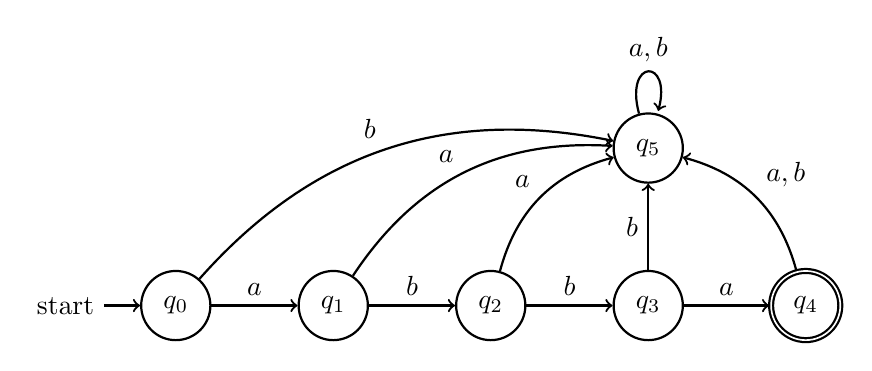
\begin{tikzpicture}[node distance=2cm, thick, auto]
% draw the states
\node[state, initial] (q_0) {\(q_0\)};
\node[state] (q_1) [right of=q_0] {\(q_1\)};
\node[state] (q_2) [right of=q_1] {\(q_2\)};
\node[state] (q_3) [right of=q_2] {\(q_3\)};
\node[state] (q_5) [above of=q_3] {\(q_5\)};
\node[state, accepting] (q_4) [right of=q_3] {\(q_4\)}; 
% draw the edges
\path[->] 
(q_0) edge node {\(a\)} (q_1)
      edge [bend left] node {\(b\)} (q_5)
(q_1) edge node {\(b\)} (q_2)
      edge [bend left] node {\(a\)} (q_5)
(q_2) edge node {\(b\)} (q_3)
      edge [bend left] node {\(a\)} (q_5)
(q_3) edge node {\(a\)} (q_4)
      edge node {\(b\)} (q_5)
(q_5) edge [loop above] node {\(a, b\)} (q_5)
(q_4) edge [bend right] node [swap] {\(a, b\)} (q_5)
;
\end{tikzpicture}
\end{document}